\begin{figure}
  \begin{subfigure}{.5\textwidth}
    \centering
    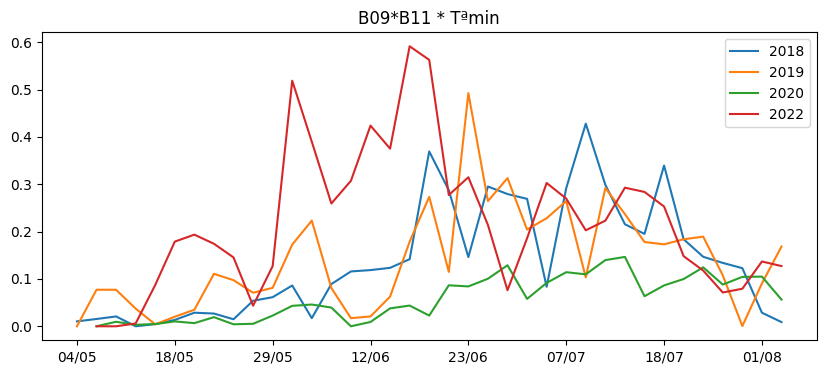
\includegraphics[width=1\linewidth]{figures/curvas_combsxTaMaxymin/0.png}
    \caption{}
  \end{subfigure}
  \begin{subfigure}{.5\textwidth}
    \centering
    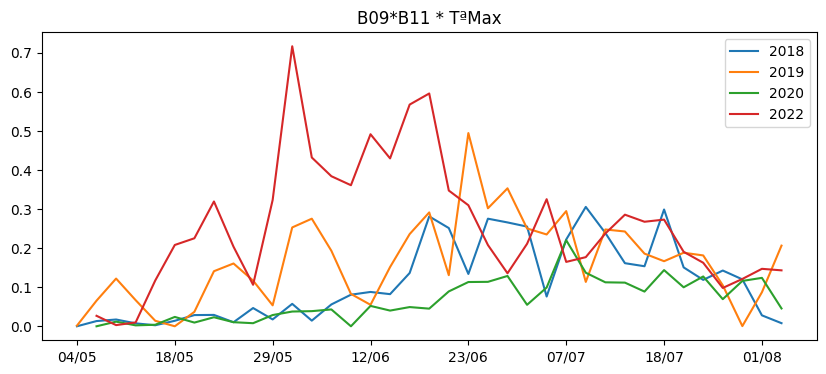
\includegraphics[width=1\linewidth]{figures/curvas_combsxTaMaxymin/1.png}
    \caption{}
  \end{subfigure}
    \caption{Progreso del producto del la Tª máxima y mínima con la reflectancia de $B_{09} * B_{11}$}
    \label{fig:curvas_combsxTaMaxymin}
\end{figure}

\begin{figure}
  \begin{subfigure}{.5\textwidth}
    \centering
    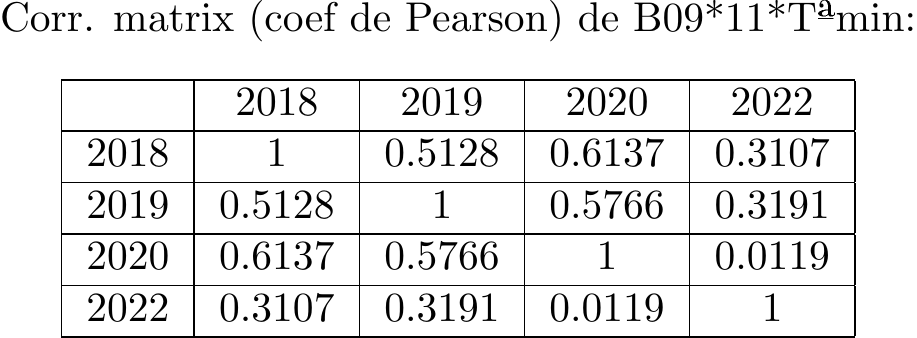
\includegraphics[width=1\linewidth]{figures/curvas_combsxTaMaxymin/tabla_0.png}
    \caption{}
  \end{subfigure}
  \begin{subfigure}{.5\textwidth}
    \centering
    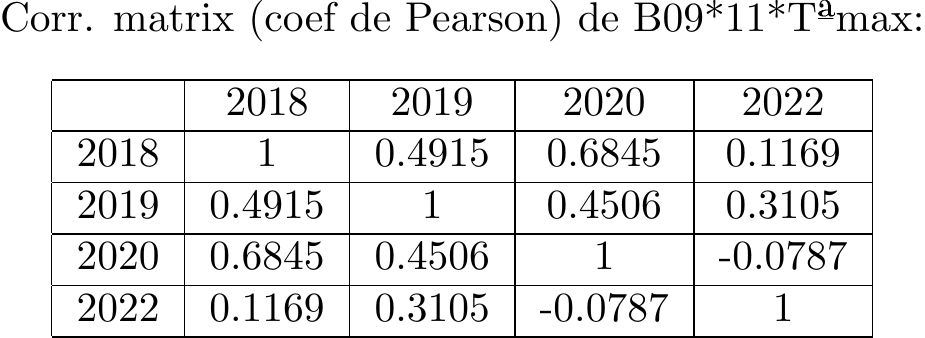
\includegraphics[width=1\linewidth]{figures/curvas_combsxTaMaxymin/tabla_1.png}
    \caption{}
  \end{subfigure}
    \caption{Correlaciones del producto del ratio $T^a_{max}/T^a_{min}$ y las reflectancias de interés}
    \label{fig:tablas_combsxTaMaxymin}
\end{figure}